\documentclass[usepdftitle=false]{beamer}
% {{{ setup
\usepackage[utf8]{inputenc}
\usepackage{tikz}
\usepackage{pgfplots}
\usepackage{isabelle,isabellesym}

\usetikzlibrary{snakes}

\useoutertheme{infolines}
\setbeamertemplate{headline}[default]
\setbeamertemplate{navigation symbols}{}

\newcommand{\Nat}{\mathbb{N}}
\newcommand{\Real}{\mathbb{R}}

% }}}

% {{{ metadata
\title[Central Limit Theorem]{A formally verified proof of the\\ Central Limit Theorem\\(preliminary report)}
\author[Avigad (CMU), \underline{H\"olzl (TUM)}, Serafin (CMU)]{%
  \begin{tabular}[t]{@{}c@{}}
    Jeremy Avigad
    \\[2ex]
    \usebeamerfont{institute}
    Carnegie Mellon University
  \end{tabular}
  \quad
  \and
  \quad
  \begin{tabular}[t]{@{}c@{}}
    \underline{Johannes H\"olzl}
    \\[2ex]
    \usebeamerfont{institute}
    TU M\"unchen
  \end{tabular}
  \and
  \quad
  \begin{tabular}[t]{@{}c@{}}
    Luke Serafin
    \\[2ex]
    \usebeamerfont{institute}
    Carnegie Mellon University
  \end{tabular}
  \vspace{-3ex}
}
\date[Isabelle Workshop 2014]{\small Isabelle Workshop 2014}

% PDF settings
\hypersetup{%
  pdftitle={A formally verified proof of the\\ Central Limit Theorem\\(preliminary report)},
  pdfauthor={Jeremy Avigad, Johannes H\"olzl, and Luke Serafin}%
}
% }}}

\begin{document}

\begingroup % {{{ titlepage
\setbeamertemplate{footline}{} % supress info footline on title page
\begin{frame}
  \maketitle
\end{frame}
\endgroup % }}}

\begin{frame}{Motivation} % {{{


\begin{center}
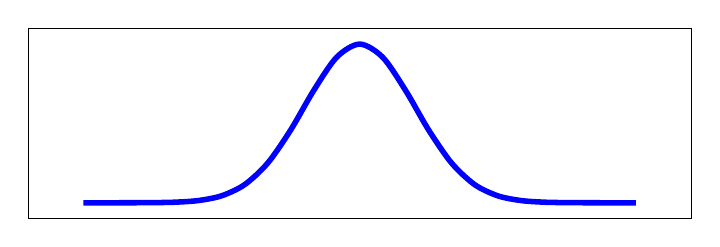
\begin{tikzpicture}
  \begin{axis}[width=10cm, height=4cm, ticks = none]
    
    \addplot[color=blue, line width = 2pt, smooth] {1 / sqrt (2 * pi) * exp(-(x ^ 2) / 2)};
    
  \end{axis}
\end{tikzpicture}
\end{center}
\begin{center} Why is the normal distribution interesting? \end{center}

\pause

\begin{center}
\Large
  The \emph{Central Limit Theorem} says that the behavior of random or chaotic events 
  becomes normal distributed when averaged over the long term. 
\end{center}

\end{frame} % }}}

\begin{frame}{Central Limit Theorem -- informal} % {{{
\begin{center} \begin{small}
$ \Pr(X_i = -1)= \frac{1}{2} \qquad \Pr(X_i = +1)= \frac{1}{2} \qquad \Pr(\sum_{i < n} X_i / \sqrt{n}) = ? $
\end{small} \end{center}

\begin{center}
\begin{tikzpicture}
  \begin{axis}[width=10cm, height=5cm,
      xmin = -5,
      xmax = 5,
      ymin = 0,
      ymax = 0.5,
      ytick = \empty,
      ybar, bar shift = {0cm},
      bar width = 2pt]
    
    \only<4,5>{\addplot[fill=red!30] table {binomial-128.dat};}
    \only<3>{\addplot[fill=red!50] table {binomial-32.dat};}
    \only<2>{\addplot[fill=red!70] table {binomial-8.dat};}
    \only<1>{
      \addplot[fill=red!90] table {binomial-2.dat};
    }
    
    \only<5>{\addplot[color=blue, line width = 2pt, smooth] {1 / sqrt (2 * pi) * exp(-(x ^ 2) / 2)};}
  \end{axis}
\end{tikzpicture}
\end{center}

\begin{center}
\only<1>{$n = 4$} \only<2>{$n = 16$} \only<3>{$n = 64$} \only<4>{$n = 256$} \only<5>{$n = \infty$}
\end{center}
\end{frame} % }}}

\begin{frame}{Central Limit Theorem -- formal} % {{{

\begin{itemize}

\item Sequence of random variables: $X : \Nat \to \Omega \to \Real$

\item $X$ are independent and identically distributed

\item Expectation: $\mathbb{E}[X_i] = 0$ and variance: $\mathbb{V}[X_i] = \sigma^2$ (for all $i$)

\end{itemize}

\[ \frac{1}{\sqrt{n \sigma^2}} \sum_{i < n} X_i ~~{\longrightarrow}_w~~ \mathcal{N}(0, 1) \]

\end{frame} % }}}

\begin{frame}{Central Limit Theorem -- in Isabelle/HOL} % {{{

\begin{isabellebody}
\isacommand{theorem}\isamarkupfalse%
\ {\isacharparenleft}\,\isakeyword{in}\ prob{\isacharunderscore}space{\isacharparenright}\ central{\isacharunderscore}limit{\isacharunderscore}theorem{\isacharcolon}\isanewline
\ \ \isakeyword{fixes}\ \isanewline
\ \ \ \ X\ {\isacharcolon}{\isacharcolon}\ {\isachardoublequoteopen}nat\ {\isasymRightarrow}\ {\isacharprime}a\ {\isasymRightarrow}\ real{\isachardoublequoteclose}\ \isakeyword{and}\isanewline
\ \ \ \ D\ {\isacharcolon}{\isacharcolon}\ {\isachardoublequoteopen}real\ measure{\isachardoublequoteclose}\ \isakeyword{and}\isanewline
\ \ \ \ {\isasymsigma}\ {\isacharcolon}{\isacharcolon}\ real\isanewline
\pause
\ \ \isakeyword{assumes}\isanewline
\ \ \ \ {\isachardoublequoteopen}indep{\isacharunderscore}vars\ {\isacharparenleft}{\isasymlambda}i{\isachardot}\ borel{\isacharparenright}\ X\ UNIV{\isachardoublequoteclose}\ \isakeyword{and}\isanewline
\ \ \ \ {\isachardoublequoteopen}{\isasymAnd}n{\isachardot}\ \alert<6>{distr}\ M\ borel\ {\isacharparenleft}X\ n{\isacharparenright}\ {\isacharequal}\ D{\isachardoublequoteclose}
\pause\ \isakeyword{and}\isanewline
\ \ \ \ {\isachardoublequoteopen}{\isasymAnd}n{\isachardot}\ integrable\ M\ {\isacharparenleft}X\ n{\isacharparenright}{\isachardoublequoteclose}\ \isakeyword{and}\isanewline
\ \ \ \ {\isachardoublequoteopen}{\isasymAnd}n{\isachardot}\ expectation\ {\isacharparenleft}X\ n{\isacharparenright}\ {\isacharequal}\ {\isadigit{0}}{\isachardoublequoteclose}
\pause\ \isakeyword{and}\isanewline
\ \ \ \ {\isachardoublequoteopen}{\isasymsigma}\ {\isachargreater}\ {\isadigit{0}}{\isachardoublequoteclose}\ \isakeyword{and}\isanewline
\ \ \ \ {\isachardoublequoteopen}{\isasymAnd}n{\isachardot}\ integrable\ M\ {\isacharparenleft}{\isasymlambda}x{\isachardot}\ {\isacharparenleft}X\ n\ x{\isacharparenright}\isactrlsup {\isadigit{2}}{\isacharparenright}{\isachardoublequoteclose}\ \isakeyword{and}\isanewline
\ \ \ \ {\isachardoublequoteopen}{\isasymAnd}n{\isachardot}\ variance\ {\isacharparenleft}X\ n{\isacharparenright}\ {\isacharequal}\ {\isasymsigma}\isactrlsup {\isadigit{2}}{\isachardoublequoteclose}\isanewline
\pause
\ \ \isakeyword{shows}\isanewline
\ \ \ \ {\isachardoublequoteopen}weak{\isacharunderscore}conv{\isacharunderscore}m\ \isanewline
\ \ \ \ \ \ \ \ {\isacharparenleft}{\isasymlambda}n{\isachardot}\ \alert<6>{distr}\ M\ \alert<6>{borel}\ {\isacharparenleft}{\isasymlambda}x{\isachardot}\ {\isasymSum}i{\isacharless}n{\isachardot}\ X\ i\ x\ {\isacharslash}\ sqrt\ {\isacharparenleft}n\ {\isacharasterisk}\ {\isasymsigma}\isactrlsup {\isadigit{2}}{\isacharparenright}{\isacharparenright}{\isacharparenright}\isanewline
\ \ \ \ \ \ \ \ {\isacharparenleft}\alert<6>{density}\ \alert<6>{lborel}\ standard{\isacharunderscore}normal{\isacharunderscore}density{\isacharparenright}{\isachardoublequoteclose}
\end{isabellebody}

\begin{visibleenv}<6->
\begin{tikzpicture}[remember picture, overlay, draw]

\node at (current page.north) [yshift=-3em, anchor=north, minimum height=5\baselineskip,
      minimum width=0.8\textwidth, fill=white, draw=red,
      thick, align=left ] {
   \texttt{distr} ::
     $\alpha\;\textit{measure} \to \beta\;\textit{measure} \to (\alpha \to \beta) \to
       \beta\;\textit{measure} $ \\
     $\texttt{distr}~\mu~\nu~f~A = \mu~\{ x \mid f\;x \in A \} $ \\[1ex]
   \texttt{density} ::
     $\alpha\;\textit{measure} \to (\alpha \to \overline{\mathbb{R}}) \to
      \alpha\;\textit{measure} $ \\
     $\texttt{density}~\mu~f~A = \int_A f\; d\mu $ \\[1ex]
   \texttt{borel} :: $\mathbb{R}~\textit{measure}$
     
     } ; 

\end{tikzpicture}
\end{visibleenv}

\end{frame} % }}}

\begin{frame}{Concepts} % {{{
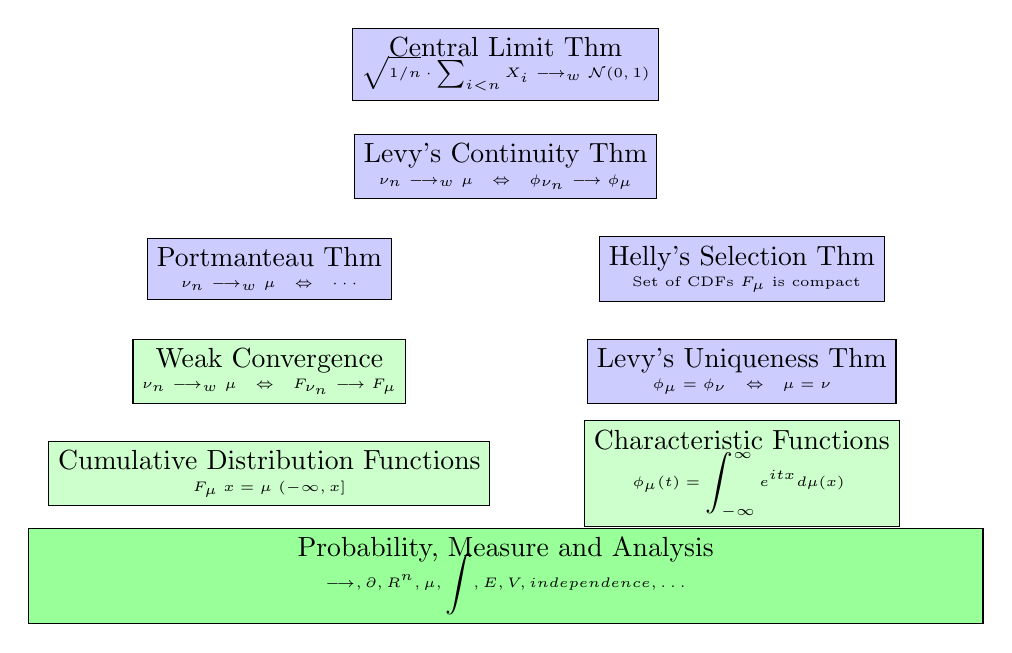
\begin{tikzpicture}[align=center, yscale=1.3,
    thm/.style={draw, fill=blue!20},
    thy/.style={draw, fill=green!20}]

  \node[draw, fill=green!40, minimum width=\textwidth] at ( 0, 0)
    { Probability, Measure and Analysis \\[-1ex] {\tiny $
      \displaystyle \longrightarrow, \partial, \mathbb{R}^n, \mu, \int, \mathbb{E}, \mathbb{V}, \text{independence}, \dots $} } ;
\pause      
  \node[thy] at (-3, 1) { Cumulative Distribution Functions \\[-1ex] {\tiny $
    F_\mu\;x = \mu~(-\infty, x] $} } ;

\pause

  \node[thy] at (-3, 2) { Weak Convergence \\[-1ex] {\tiny $
    \nu_n ~ {\longrightarrow}_w ~ \mu ~~\Leftrightarrow~~ F_{\nu_n} \longrightarrow F_\mu $} } ;

\pause

  \node[thm] at (-3, 3) { Portmanteau Thm \\[-1ex] {\tiny $
    \nu_n ~ {\longrightarrow}_w ~ \mu ~~ \Leftrightarrow ~~ \cdots $} } ;

\pause

  \node[thy] at ( 3, 1) { Characteristic Functions \\ {\tiny $\displaystyle
    \phi_\mu(t) = \int_{-\infty}^{\infty} e^{itx} d\mu(x) $ } } ;

  \node[thm] at ( 3, 2) { Levy's Uniqueness Thm \\[-1ex] {\tiny $
    \phi_\mu = \phi_\nu ~~ \Leftrightarrow ~~ \mu = \nu $ }} ;

\pause

  \node[thm] at ( 3, 3) { Helly's Selection Thm \\[-1ex] { \tiny
    Set of CDFs $F_\mu$ is compact }} ;

  \node[thm] at ( 0, 4) { Levy's Continuity Thm \\[-1ex] {\tiny $
    \nu_n~{\longrightarrow}_w~\mu ~~\Leftrightarrow~~ \phi_{\nu_n} \longrightarrow \phi_\mu $} } ;

\pause

  \node[thm] at ( 0, 5) { Central Limit Thm \\[-1ex] {\tiny $
    \sqrt{1/n} \cdot \sum_{i<n} X_i ~ {\longrightarrow}_w ~ \mathcal{N}(0,1) $} } ;

\end{tikzpicture}
\end{frame} % }}}

\begin{frame}{Weak convergence of measures (I)} % {{{

\begin{center}
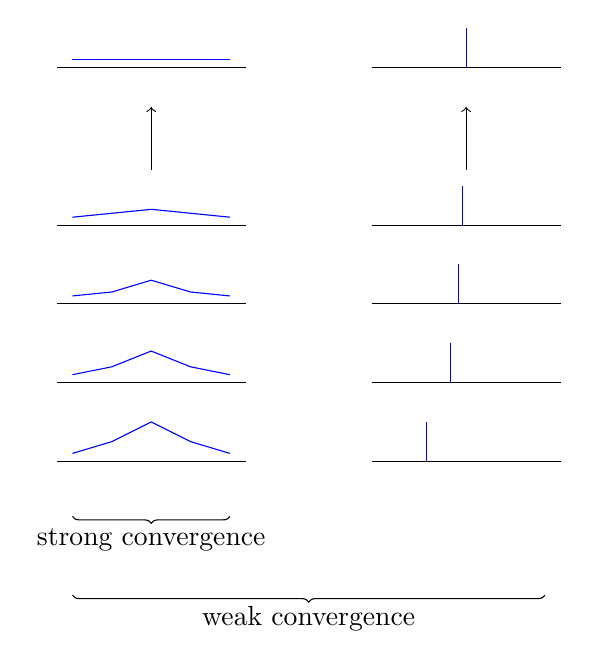
\begin{tikzpicture}

\onslide<1->{
\begin{scope}[yshift=1cm]
  \draw (-1.2, 0) -- (1.2, 0) ;
  \draw[blue] (-1, 0.1) -- (-0.5, 0.25) -- (0, 0.5) -- (0.5, 0.25) -- (1, 0.1) ;
\end{scope}     

\begin{scope}[yshift=2cm]
  \draw (-1.2, 0) -- (1.2, 0) ;
  \draw[blue] (-1, 0.1) -- (-0.5, 0.20) -- (0, 0.4) -- (0.5, 0.20) -- (1, 0.1) ;
\end{scope}

\begin{scope}[yshift=3cm]
  \draw (-1.2, 0) -- (1.2, 0) ;
  \draw[blue] (-1, 0.1) -- (-0.5, 0.15) -- (0, 0.3) -- (0.5, 0.15) -- (1, 0.1) ;
\end{scope}

\begin{scope}[yshift=4cm]
  \draw (-1.2, 0) -- (1.2, 0) ;
  \draw[blue] (-1, 0.1) -- (-0.5, 0.15) -- (0, 0.2) -- (0.5, 0.15) -- (1, 0.1) ;
\end{scope}

\begin{scope}[yshift=6cm]
  \draw (-1.2, 0) -- (1.2, 0) ;
  \draw[blue] (-1, 0.1) -- (-0.5, 0.10) -- (0, 0.1) -- (0.5, 0.10) -- (1, 0.1) ;
\end{scope}

\draw [->] (0, 4.7) -- (0, 5.5) ;

\draw[snake=brace] (1, 0.3) -- (-1, 0.3) ;

\node at (0, 0) { strong convergence } ;
}

\onslide<2->{
\begin{scope}[yshift=1cm, xshift=4cm]
  \draw (-1.2, 0) -- (1.2, 0) ;
  \draw[blue] (-0.5, 0.0) -- (-0.5, 0.5) ;
\end{scope}     

\begin{scope}[yshift=2cm, xshift=4cm]
  \draw (-1.2, 0) -- (1.2, 0) ;
  \draw[blue] (-0.2, 0.0) -- (-0.2, 0.5) ;
\end{scope}

\begin{scope}[yshift=3cm, xshift=4cm]
  \draw (-1.2, 0) -- (1.2, 0) ;
  \draw[blue] (-0.1, 0.0) -- (-0.1, 0.5) ;
\end{scope}

\begin{scope}[yshift=4cm, xshift=4cm]
  \draw (-1.2, 0) -- (1.2, 0) ;
  \draw[blue] (-0.05, 0.0) -- (-0.05, 0.5) ;
\end{scope}

\begin{scope}[yshift=6cm, xshift=4cm]
  \draw (-1.2, 0) -- (1.2, 0) ;
  \draw[blue] (0, 0.0) -- (0, 0.5) ;
\end{scope}

\draw [->] (4, 4.7) -- (4, 5.5) ;

}

\onslide<3->{
\draw[snake=brace] (5, -0.7) -- (-1, -0.7) ;
\node at (2, -1) { weak convergence } ;
}

\end{tikzpicture}
\end{center}

\end{frame}

\begin{frame}{Weak convergence of measures (II)} % {{{

\begin{definition}[Cumulative Distribution Function]%
\vspace{-2ex}
\begin{center}%
$ F_\mu~x := \mu~(-\infty, x] $
\end{center}
{($\approx 320$ lines of thy, uniqueness, char. and right-cont. monotone func.)}
\end{definition}

\pause

\begin{definition}[Weak convergence]
\vspace{-2ex}
\begin{center} 
$ \begin{array}{l} \nu_n ~{\longrightarrow}_w~ \mu :\Leftrightarrow \\
\qquad
  (\forall t.~ F_\mu~\text{continuous at}~ t \implies
       F_{\nu\,n}~t \longrightarrow F_\mu~t)
  \end{array} $
\end{center}
\end{definition}

\pause

\begin{theorem}[Portmanteau Theorem]
Equivalent characterizations of $\nu_n ~{\longrightarrow}_w~ \mu$:
\begin{itemize}
 \item $\int f \; d\nu_n \longrightarrow \int f \; d\mu$ ~~ for every bounded, continuous $f$
 \item $\nu_n~A \longrightarrow \mu_n~A$ ~~ for all Borel sets $A$, with $\mu(\partial A) = 0$
\end{itemize}
\end{theorem}

($\approx 900$ lines of thy)

\end{frame} % }}}


\begin{frame}{Characteristic functions} % {{{

\begin{definition}[Characteristic functions]%
\vspace{-1em}
\begin{center} $ \displaystyle \phi_\mu~t = \int_{-\infty}^{\infty} e^{itx} d\mu(x) $ \end{center}
\end{definition}

\pause

\begin{theorem}[Levy Uniqueness Theorem]
\vspace{-1em}
\begin{center} $ \phi_{\mu_1} = \phi_{\mu_2} \Leftrightarrow \mu_1 = \mu_2 $ \end{center} 
\end{theorem}

\pause

\begin{theorem}[Levy Continuity Theorem]
\vspace{-1em}
\begin{center} $ \nu_n ~{\longrightarrow}_w~ \mu \Leftrightarrow
  (\forall t.\ \phi_{\nu_n}~t \longrightarrow \phi_\mu~t) $ \end{center}
\end{theorem}

\pause

Also the characteristic function of the std. normal distribution:
\[ \phi_{\mathcal{N}(0, 1)}~t = e^{-t^2/2}\]

($\approx 3\,000$ lines of thy)
\end{frame} % }}}

\begin{frame}{Central Limit Theorem -- the proof} % {{{
\begin{itemize}[<+->]

  \item Show: $S_n ~{\longrightarrow}_w~ \mathcal{N}(0, 1)$ where $S_n = \frac{1}{\sqrt{n\cdot \sigma^2}} \sum_{i < n} X_i$

  \item With Levy's Continuity Theorem:
    $\phi_{S_n}~t \longrightarrow \phi_{\mathcal{N}(0, 1)}~t$
    
  \item We have $\phi_{\mathcal{N}(0, 1)}~t = e^{-t^2/2}$
  
  \item We have $\phi_{S_n}~t \approx
    (1 + \frac{- t^2 / 2}{n})^n$
  
  \item Power series approximation of the exponential function:
    $(1 + \frac{- t^2 / 2}{n})^n \longrightarrow e^{-t^2/2}$ \\

  \onslide<6->{\qed}
\end{itemize}

\uncover<7>{
\begin{center}
  Size of the final CLT proof: 120 lines of theory
\end{center}}
\end{frame} % }}}

\begin{frame}

What was missing?

\begin{itemize}
\item Lebesgue integration slightly insufficent: \\
  No support set ($\int_A f\;d\mu$); only $\mathbb{R}$-valued functions
\pause
\item Complex analysis (characterisitic function of the normal distribution)
\pause

\item Various smaller theorems about limits of transcendental functions
\pause

\item Interval integral, i.e. to deal with: $\int_{a}^b f\; d\mu, \int_{a}^\infty f\; d\mu, \int_{\infty}^b f\; d\mu, \ldots$

\end{itemize}

\pause

Material already moved to or changed in Isabelle/HOL:

\begin{itemize}

\item Introduce Bochner integration (unifies integration of $\mathbb{R}$ and $\mathbb{C}$): \\
  From $\int {f}\; d\!\mu :: \mathbb{R}$ to $\int {f}\; d\!\mu :: \mathbb{R}^n$

\pause

\item Definition of the Lebesgue-Stieltjes measure: \\ 
  $\mathcal{L}_F~[a, b] = F~b - F~a$

\pause

\item Moments of the normal distribution ($\mathbb{E}[X^n]$)

\pause

\item A lot of small theorems about limits, uncountable sets, $\dots$

\pause

\item Set based integral $\int_A f\;d\mu$, and interval integral not moved yet

\end{itemize}

\end{frame}

\begin{frame}{Summary} % {{{
\begin{itemize}

\item Current size: $\approx 6\,250$ lines of thy\\
  (After cleanup etc., paper mentions $\approx 13\,000$ lines)

\pause

\item CLT fundamental to contemporary probability theory

\pause

\item The necessary machinery (characterisitic functions, weak convergence) is in itself important

\item The proofs can be found online at \url{https://github.com/avigad/isabelle}

\end{itemize}


\begin{center} \LARGE Questions? \end{center}

\end{frame} % }}}

\end{document}
